%% May 2016, 
%presentation inspired by the presentation made in CAA, the presentation made at the Winter Simulation Conference, and some ideas tooks from #RIN4 at the UPF

\documentclass[12pt, notes=show]{beamer}
\usetheme[width=0cm]{Goettingen}
\usecolortheme{rose}
\useoutertheme{default}
\setbeamerfont{caption}{size=\scriptsize}
\setbeamertemplate{navigation symbols}{}

\addtobeamertemplate{navigation symbols}{}{%
	\usebeamerfont{footline}%
	\usebeamercolor[fg]{footline}%
	\hspace{1em}%
	$\dfrac{\insertframenumber}{\inserttotalframenumber}$
}

\usepackage{hyperref}
\usepackage{fontspec} 
\setsansfont{Futura LT}


\usepackage{arydshln}
\usepackage{amsmath}

\usepackage{mathptmx}
\usepackage{latexsym}
\usepackage{mathtools}
\usepackage{multirow}
\usepackage{caption}



\title{
	BSC Symposium:\\
	Co-evolution of trade and culture.
}

\institute{May 2016}

\author{Simon Carrignon, Jean-Marc Montanier \& Xavier Rubio-Campillo}

\date{
	\scriptsize
	\begin{columns}
		\begin{column}{.3\textwidth}
			\begin{center}
				Barcelona Supercomputing Center	\\
				
\includegraphics[height=1cm]{images/bscLogo.jpg} \hspace{2cm}
			\end{center}
		\end{column}
		\begin{column}{.3\textwidth}
			\begin{center}
				Univ. Pompeu Fabra Complex System Lab.\\
				\includegraphics[height=1cm]{images/upfLogo.jpeg} %declare logo image with an alias here 
			\end{center}
		\end{column}
	\end{columns}

}
\begin{document}
\begin{frame}
	\maketitle

\end{frame}

%\begin{frame}{Plan of the presentation}
%	\begin{enumerate}
%		\item Introduction
%			\vfill
%		\item Model Description \& Tests
%			\vfill
%		\item Future Works
%			\vfill
%	\end{enumerate}
%	
%\end{frame}

\section{Introduction}

\begin{frame}{Cultural Evolution}
    Social Traits:
    \begin{center}
	\begin{table}
	    \center
	    \begin{tabular}{ccc}
		\uncover<2->{\includegraphics[height=3cm]{images/m80}} &
		\uncover<3->{\includegraphics[height=3cm]{images/m90}} &
		\uncover<4->{\includegraphics[height=3cm]{images/m10}} \\
		\uncover<2->{80's} & \uncover<3->{90's} & \uncover<4->{now}
	    \end{tabular}
	\end{table}
    \end{center}
    \uncover<5->{How they Evolve?}\uncover<6>{ Cultural Evolution }
\end{frame}

%\begin{frame}
%
%    \invisible<2>{This text will be invisible on slide 2, but not on others slides}\\
%    This text is always visible\\
%    \uncover<1->{Beamer} \uncover<2->{is}  \uncover<3->{super} \uncover<4->{powerful} 
%
%\end{frame}
%\begin{frame}
%
%    \begin{itemize}
%	\item em Language used by Beamer: L\uncover<2->{A}TEX
%	\item em Language used by Beamer: L\only<2->{A}TEX
%    \end{itemize}
%
%\end{frame}

\begin{frame}{Cultural Evolution}
    \begin{itemize}
	\item<5->{ culturally transmitted, socially learnt}
	\item<6->{ similar patterns}
    \end{itemize}
	\begin{center}
		\uncover<4->{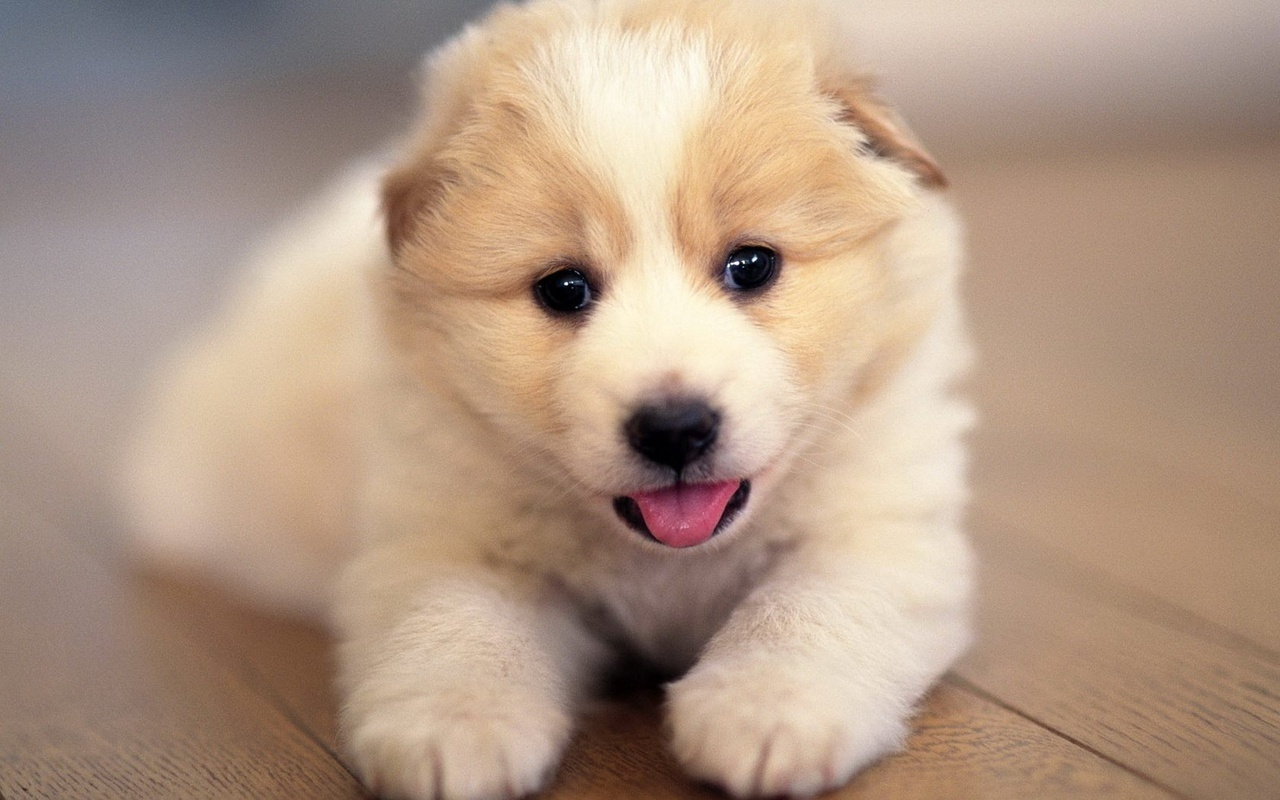
\includegraphics[width=3cm]{images/cutdog}}\\
		\vspace{.5cm}
		\uncover<2->{\includegraphics[width=2.5cm]{images/cutbaby}}
	    \hspace{1cm}
	    \uncover<3->{ \includegraphics[width=2cm]{images/pottery}}
	\end{center}
    \uncover<7>{$\rightarrow$ What mechanism drive the evolution of such traits?\\
    \invisible<1->{$\rightarrow$ What mechanism }generate such pattern?}
\end{frame}

\begin{frame}{What Generate Those Cultural changes?}
	Simple mechanisms (Bentley et al, 2004):
	\begin{itemize}
		\item<2->Random Copy 
		\item<3-> Frequency biased (conformist/anti-conformist\dots)
		\item<4->\dots	
	\end{itemize}
	\uncover<2>{\begin{figure}
		\begin{columns}
			\begin{column}{.8\textwidth}
				\centering
				\includegraphics[width=.6\textwidth]{images/powerlawrepartition.jpg}
			\end{column}
			\begin{column}{.3\textwidth}
				\tiny
				Square: male names\\
				Circle: female names\\
				Dotted and plain lines: model result with different copy probabilities.\\
			From Bentley et al,~2004.
			\end{column}
		\end{columns}
	    \end{figure}}
\end{frame}

\section{Context}


\begin{frame}
	\begin{center}
	    What if such mechanisms act on traits linked to economics?
	\end{center}
	\begin{center}
	    \only<2>{\vspace{1cm}\includegraphics[height=3cm]{images/bordeaux.jpg}\hspace{2cm}
	    \includegraphics[height=3cm]{images/napa}}
	    \only<3>{\includegraphics[height=4cm]{images/tools}}
	    \only<4>{\includegraphics[height=4cm]{images/stockoption}}
	\end{center}
\end{frame}

%Next slide was bad
%\begin{frame}
%	\begin{columns}
%		\begin{column}{.3\textwidth}
%			\includegraphics[width=\textwidth]{images/bordeaux.jpg}	
%		\end{column}
%
%		\begin{column}{.2\textwidth}
%		\end{column}
%		\begin{column}{.3\textwidth}
%			\includegraphics[width=3cm]{images/napa}	
%		\end{column}
%	\end{columns}
%	\begin{center}
%		What happen when such mechanisms act on traits impacting economy?
%	\end{center}
%	\begin{columns}
%		\begin{column}{.3\textwidth}
%			\includegraphics[width=\textwidth]{images/tools}	
%		\end{column}
%		\begin{column}{.2\textwidth}
%		\end{column}
%		\begin{column}{.3\textwidth}
%			\includegraphics[width=3cm]{images/stockoption}	
%		\end{column}
%	\end{columns}
%\end{frame}
%
\begin{frame}{Co-evolution of Economy and Culture}

%How Simple Cultural Dynamics influence Economy That in turn will influence cultural dynamics.
    \begin{center}
	\includegraphics[width=\textwidth]{images/interaction}	
    \end{center}

\end{frame}

\section{ABM Framework}

%\begin{frame}{A General Agent Based Framework }
%	\begin{center}
%	    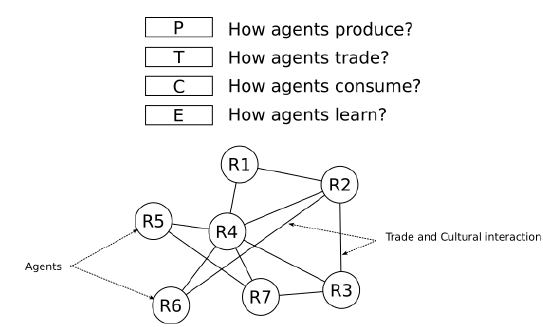
\includegraphics[width=.6\textwidth]{images/schema_model.png}
%	\end{center}
%\end{frame}

%Slide xavi wanted me to put but I cannot make it fit
\begin{frame}{Material}
Usually, to perform such study:\\
	Facebook, twitter, database of photos\dots\\
	    \vspace{.5cm}
	    \begin{alertblock}{Biases} 
	Comparison between cultures and across time is needed : \\
	    \begin{center}
		\uncover<2>{\large \textbf{Archaeology}}
	    \end{center}
	
    \end{alertblock}
\end{frame}

\begin{frame}
    \centering
    \Large
    Our Model
\end{frame}

\begin{frame}{A General Agent Based Framework }

     Two main components:
     \vfill
    \begin{enumerate}
	\item Trade side: Bartering Economy (Gintis 2009),
	\item Cultural side: ``copy the most successful'' (Bentley 2006).
    \end{enumerate}
    \begin{center}
	\includegraphics[width=.8\textwidth]{images/interaction}	
    \end{center}
\end{frame}
	

\begin{frame}{The Model}
	\begin{block}{1. The Economy \& the Barter Mechanism}
		\begin{itemize}
			\item $N$ goods
			\item $M$ Agent 
				$\left\{
					\begin{tabular}{@{}l@{}}
						a quantity of each Goods \\
						$N$ values attributed to each goods\\
					\end{tabular}
					\right.$
				\item Agents \emph{produce} one good and \emph{exchange} it to obtain the other goods.
				\item After the exchange, the agents \emph{consume} all goods 
			\end{itemize}
			Agent perform this 10 times and a scores is given to each of them.
		\end{block}
	\end{frame}

	\begin{frame}{The Model}
		\begin{block}{2. Cultural Mechanisms}
			\begin{itemize}
					\vfill
				\item Less successful agents \emph{copy} the most successful (Biased-Copy).
					\vfill
				\item Given a probability $\mu$ the value attributed to some goods is modified (Innovation/Mutation)
			\end{itemize}
		\end{block}
	\end{frame}
\begin{frame}{Experiments}
	\centering
	\textbf{Trade Model} \\Trade Mechanism + Success Biased Copy\\
	\vfill
	vs\\
	\vfill
	\textbf{Neutral Model}\\ Trade Mechanism + Random Copy\\
	 

\end{frame}


\section{Results}

\begin{frame}{Results: Frequency Distribution}
    \subsection*{Distribution of variant:}
    \begin{figure}[!h]
	\begin{center}
	    \begin{tabular}{ccc}
		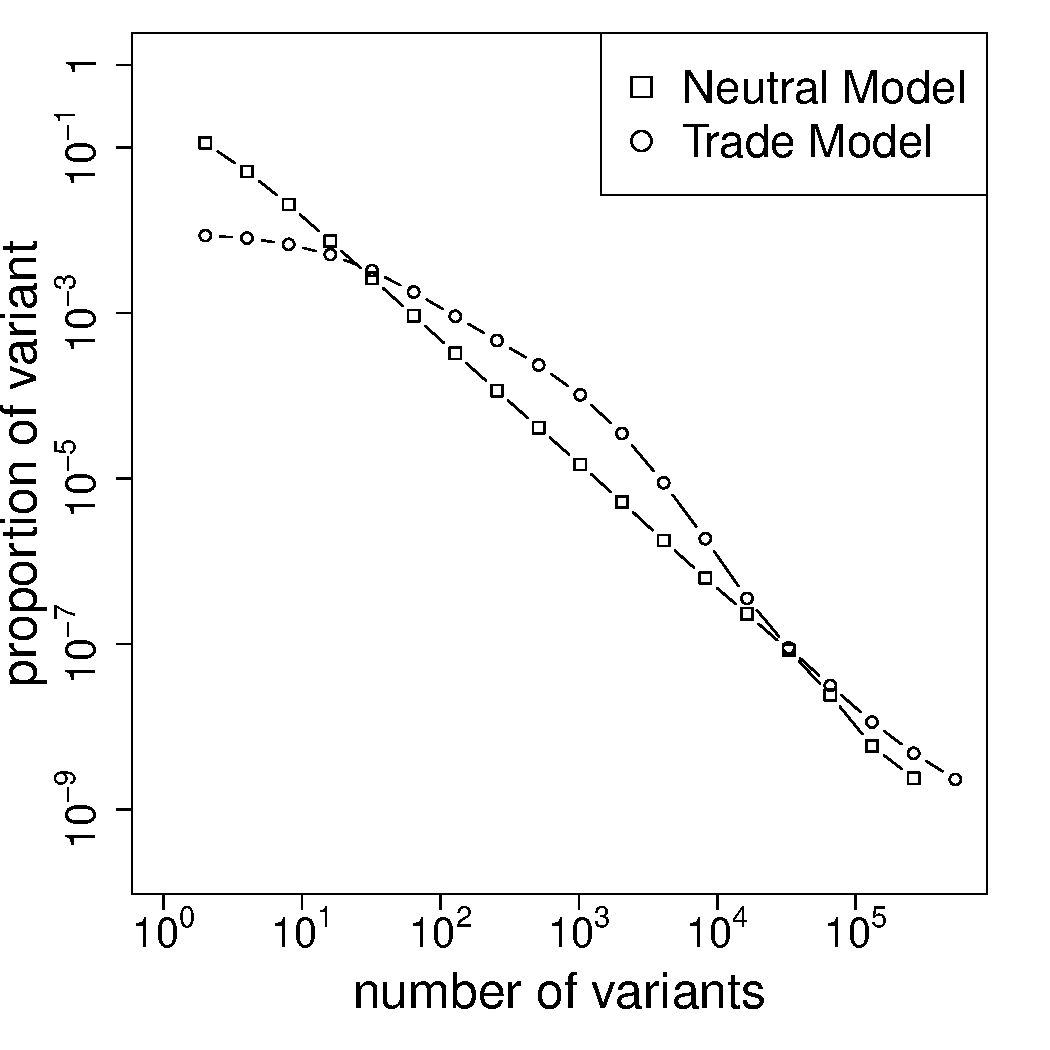
\includegraphics[width=5cm]{images/2SetupDistribA.pdf}\\
	    \end{tabular}

	\end{center}
	%\caption{Frequencies distribution, where each points represent the mean for 100 runs, for: a) the neutral and the trading models.  b) the neutral model and the trading model without the trading innovation process. c) the trade model and the trade model without the trading innovation process.}
    \end{figure}
\end{frame}


\begin{frame}{Results: Economic Dynamic}
    \begin{figure}[!h]
	\centering
	\begin{tabular}{ c c}
	    Neutral Model & Trading Model \\
	    \includegraphics[width=5cm]{images/ScoreEvolutionForRandom-G3N500.pdf}
	    & 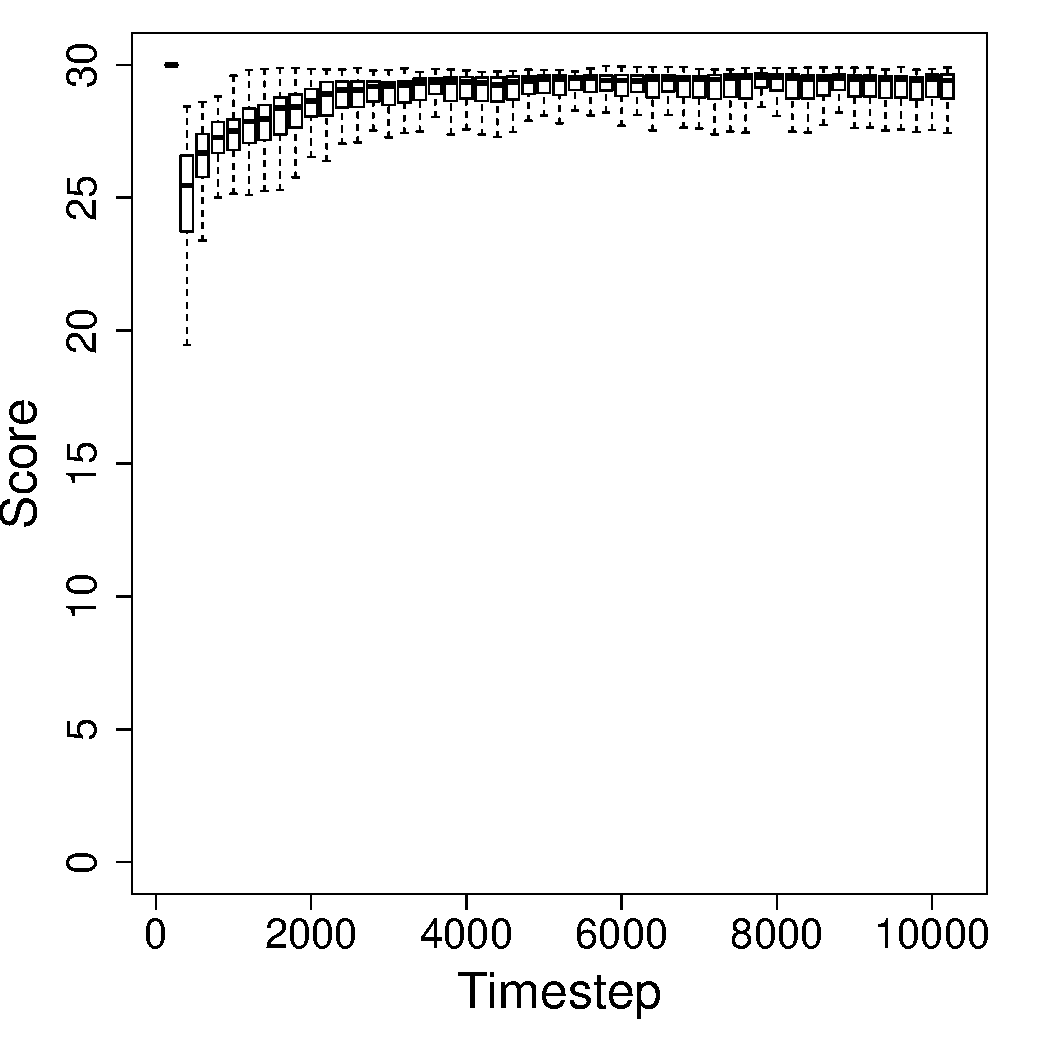
\includegraphics[width=5cm]{images/ScoreEvolutionForTrade-G3N500.pdf}

	\end{tabular}
	\caption{Evolution of the score within the two different models for two typical run with 500 agents and 3 goods evolving during 10000 timestep.}%%
	\label{fig:scoreEvol}
    \end{figure}
\end{frame}
    


\begin{frame}{Results: Economic Dynamics}
	\begin{figure}
	    \caption{Example for 3 goods and 500 agents}
	    \begin{columns}
		\column{.5\textwidth}
		\includegraphics[height=\textwidth]{images/ClearingPriceDistanceEvolutionForTrade-G3N500.pdf}\\
	    \end{columns}
		@~Equilibrium: personal values  $\rightarrow$ optimal (shared) values.
	\end{figure}
	
\end{frame}

\begin{frame}{Summary}
\begin{itemize}
		\vfill
	    \item Economic Dynamic $\rightarrow$ Culture :
			\begin{itemize}
			    \item Random social learning: scale-free distribution of trait. 
			    \item Social learning biased toward economic attribute: non power-law distribution.
			\end{itemize}
		\vfill
	    \item Culture Mechanism $\rightarrow$ Economy : 
		\begin{itemize}
		    \item Random Mechanism: inefficient eco.
		    \item Biased Mechanism: efficient eco.
		\end{itemize}
		\vfill
	\item A local copy mechanism alone is enough to bring the global economy to an optimal equilibrium.
\end{itemize}

\end{frame}
\section{Application}
\begin{frame}{Next Objectives}
    \vfill
    Understand general dynamics and properties of such systems:
    \vfill
	\begin{itemize}
	\item Different Cultural Mechanisms
    \vfill
	\item Different Trade Assumption
    \vfill
	\item Network Constraints
    \vfill
	\item \dots
    \vfill
	\end{itemize}
\end{frame}

\begin{frame}{}

    {\large Study Cultural evolution \textbf{is not} possible without archaeology studies}
    \vspace{.5cm}
    \uncover<2->{
    \begin{center}
	and
    \end{center}
    \vspace{.5cm}
}

\uncover<3>{    {\large Simulation as a tool to implement and test hypothesis made on Historical questions.}\\
    \vspace{.5cm}
	{\scriptsize(Carrignon et al., Model \& Simluation 7, May 2016, BCN)}
    }
	
\end{frame}

\begin{frame}{Case Study}

    \begin{columns}
	\begin{column}{.35\textwidth}
	The Economy of the Roman Empire \\
	\end{column}
	\begin{column}{.6\textwidth}
	\begin{figure}
	    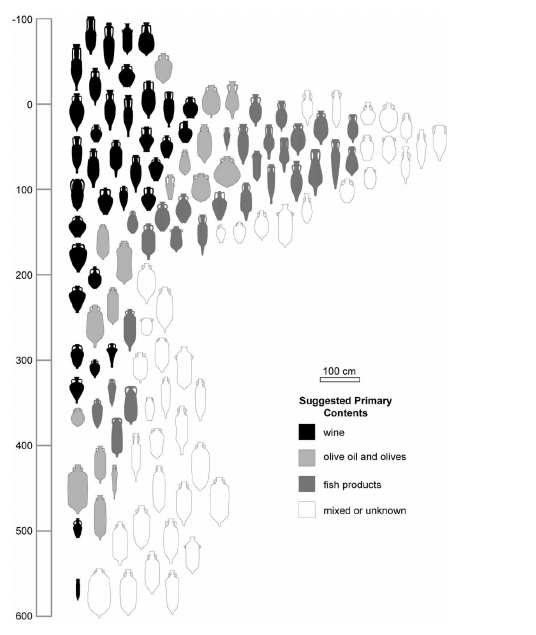
\includegraphics[width=\textwidth]{images/bevan.png}\\
	\caption{\scriptsize Bevan 2014}
	\end{figure}
	\end{column}
    \end{columns}
\end{frame}

\begin{frame}
    %{Case Study}
	\begin{center}
		\Large
    Thank for you attention!\\
%		What was the nature of Roman economy?\\
		\includegraphics[width=2cm]{images/LOGO-ERC.jpg} \hfil	\includegraphics[width=3cm]{images/epnetLogo.png}\\
		\vspace{1cm}
		\scriptsize
			http://www.roman-ep.net/\\
			@epnetproject\\
			fb.com/EPNetProject\\
			@simoncarrignon
	\end{center}


\end{frame}

%\begin{frame}
%    \Huge
%    Thank for you attention!
%\end{frame}
\end{document}


